% ------------------------------------------------------------------------
% ------------------------------------------------------------------------
% abnTeX2: Modelo de Trabalho Academico (tese de doutorado, dissertacao de
% mestrado e trabalhos monograficos em geral) em conformidade com 
% ABNT NBR 14724:2011: Informacao e documentacao - Trabalhos academicos -
% Apresentacao
% ------------------------------------------------------------------------
% ------------------------------------------------------------------------

\documentclass[
	% -- opções da classe memoir --
	12pt,				% tamanho da fonte
	openright,			% capítulos começam em pág ímpar (insere página vazia caso preciso)
	oneside,			% para impressão em verso e anverso. Oposto a oneside
	a4paper,			% tamanho do papel. 
	% -- opções da classe abntex2 --
	chapter=TITLE,		% títulos de capítulos convertidos em letras maiúsculas
	section=TITLE,		% títulos de seções convertidos em letras maiúsculas
	%subsection=TITLE,	% títulos de subseções convertidos em letras maiúsculas
	%subsubsection=TITLE,% títulos de subsubseções convertidos em letras maiúsculas
	% -- opções do pacote babel --
	english,			% idioma adicional para hifenização
	french,				% idioma adicional para hifenização
	spanish,			% idioma adicional para hifenização
	brazil				% o último idioma é o principal do documento
	]{abntex2}

% ---
% PACOTES
% ---

% ---
% Pacotes fundamentais 
% ---
%\usepackage{lmodern}			% Usa a fonte Latin Modern			
\usepackage{times}				% Usa a fonte Times
\usepackage[T1]{fontenc}		% Selecao de codigos de fonte.
\usepackage[utf8]{inputenc}		% Codificacao do documento (conversão automática dos acentos)
\usepackage{lastpage}			% Usado pela Ficha catalográfica
\usepackage{indentfirst}		% Indenta o primeiro parágrafo de cada seção.
\usepackage{color}				% Controle das cores
\usepackage{graphicx}			% Inclusão de gráficos
\usepackage{microtype} 			% para melhorias de justificação
\usepackage{listings}			% para inserir código fonte
\usepackage{float}				% para garantir que as figuras fiquem no mesmo lugar em que foram inseridas
\usepackage{caption}			% para utilizar \captionsetup e remover figuras do apêndice da lista

% Correção da separação de palavras separadas erroneamente ou que desalinham o texto também
\hyphenation{bio-mé-tri-ca}

% ---
% Pacotes de citações
% ---
\usepackage[alf,abnt-year-extra-label=yes,abnt-emphasize=bf, bibjustif]{abntex2cite}	% Citações padrão ABNT
\usepackage{titlesec}

% --- 
% CONFIGURAÇÕES DE PACOTES
% --- 

% altera o espacamento depois do número de cada secao, subsecao, etc
\titleformat{\section}
  {\normalfont\normalsize\uppercase}{}{0pt}{\thesection\space}
\titleformat{\subsection}
  {\normalfont\normalsize\bfseries}{}{0pt}{\thesubsection\space}
\titleformat{\subsubsection}
  {\normalfont\normalsize}{}{0pt}{\thesubsubsection\space}
\titleformat{\paragraph}
  {\normalfont\normalsize\itshape}{}{0pt}{\theparagraph\space}

%% para ajudar na revisao do texto
\usepackage[normalem]{ulem}
\definecolor{comentCor}{rgb}{1,0,0}
\newcommand{\ignore}[1]{\textcolor{red}{\sout{#1}}}
\newcommand{\coment}[1]{\textcolor{comentCor}{Revisor: #1}}
% ---

% ---
% **************************************************
% Informações que devem ser alteradas
% **************************************************
\titulo{\uppercase{Título do TCC}}
\autor{\uppercase{Autor 1} \\
		\uppercase{Autor 2} \\
		\uppercase{Victor Paranhos}}
\orientador{Nome do Orientador}
\orientadortcc{Prof. \imprimirorientador, MSc. \\ Universidade Anhembi Morumbi}
\coordenador{Nome do Coordenador do Curso}
\coordenadortcc{Nome do Coordenador}
\examinador{Nome do Convidado \\ Universidade Anhembi Morumbi}
\preambulo{Trabalho de Conclusão de Curso apresentado como exigência parcial para a obtenção do título de Bacharel em Sistemas de Informação da Universidade Anhembi Morumbi, sob a orientação do Prof. MSc. \imprimirorientador.}
\proforientador{Orientador: \imprimirorientador.}
\datadefesa{\uppercase{}} %00 de Junho de 2016
\local{São Paulo/SP}
\data{2016}
% **************************************************

\instituicao{
  UNIVERSIDADE ANHEMBI MORUMBI
  }
\tipotrabalho{Trabalho de Conclusão de Curso}

% alterando o aspecto da cor azul
\definecolor{blue}{RGB}{41,5,195}

% informações do PDF
\makeatletter
\hypersetup{
     	%pagebackref=true,
		pdftitle={\@title}, 
		pdfauthor={\@author},
    	pdfsubject={TCC S.I.},
	    pdfcreator={\@author},
		pdfkeywords={\@title}, 
		colorlinks=true,      	% false: boxed links; true: colored links
		linkcolor=black,	% color of internal links
		citecolor=black,        % color of links to bibliography
		filecolor=magenta,      % color of file links
		urlcolor=black,
		bookmarksdepth=4
}
\makeatother
% --- 

% --- 
% Espaçamentos entre linhas e parágrafos 
% --- 

% O tamanho do parágrafo é dado por:
\setlength{\parindent}{1.3cm}

% Controle do espaçamento entre um parágrafo e outro:
\setlength{\parskip}{0.2cm}  % tente também \onelineskip

%\titlespacing\section{0pt}{12pt plus 4pt minus 2pt}{-6pt plus 2pt minus 2pt}

% ---
% compila o indice
% ---
\makeindex
% ---

% ----
% Início do documento
% ----
\begin{document}

% Retira espaço extra obsoleto entre as frases.
\frenchspacing 

% ----------------------------------------------------------
% ELEMENTOS PRÉ-TEXTUAIS
% ----------------------------------------------------------

\imprimircapa
\imprimirfolhaderosto*

\begin{folhadeaprovacao}

	\begin{center}
    	{\ABNTEXchapterfont\bfseries\normalsize\textnormal\imprimirautor}

    	\vspace*{\fill}
    	
    	\begin{center}
      		\ABNTEXchapterfont\bfseries\normalsize\imprimirtitulo
    	\end{center}
        \hspace{.45\textwidth}
      	\begin{minipage}{.5\textwidth}
      		\SingleSpacing
         	\imprimirpreambulo
       	\end{minipage}
        
   		\begin{flushleft}	
   			Aprovado em: {\imprimirdatadefesa}
   		\end{flushleft}
   		
   		\assinatura{\imprimirorientadortcc} 
   		\assinatura{\imprimirexaminador}
   		\assinatura{\imprimirexaminador}
	\end{center}

\end{folhadeaprovacao}

% Arquivos que devem ser alterados
% ====================================================================
% Dedicatória 
% ====================================================================
\begin{dedicatoria}
	\vspace*{\fill}
	\vspace*{\fill}
	\begin{flushright}
		Este trabalho é dedicado aos que acreditam...
	\end{flushright}
	\vspace*{\fill}
\end{dedicatoria}

% ====================================================================
% Agradecimentos 
% ====================================================================
\begin{agradecimentos}
	Agradecimentos devem ser escritos aqui.
\end{agradecimentos}

% ====================================================================
% Epigrafe 
% ====================================================================
\begin{epigrafe}
    \vspace*{\fill}
    \vspace*{\fill}
	\begin{flushright}
		\textit{``Inteligência é a habilidade de evitar fazer o trabalho, \\
		e mesmo assim conseguir ter o trabalho realizado.''} \\
		(Linus Torvalds)
	\end{flushright}
	\vspace*{\fill}
\end{epigrafe}


% ====================================================================
% Resumo 
% ====================================================================


\setlength{\absparsep}{18pt} % ajusta o espaçamento dos parágrafos do resumo
\begin{resumo}
	O resumo deve ser escrito aqui.

 PALAVRAS-CHAVE: Palavra Chave. Teste. Universidade Anhembi Morumbi.
\end{resumo}

% ====================================================================
% Abstract 
% ====================================================================
\begin{resumo}[\textbf{ABSTRACT}]
 \begin{otherlanguage*}{english}
   Abstract must be written here.

   \vspace{\onelineskip}
 
   \noindent 
   \textbf{KEYWORDS}: Keyword. Test. Universidade Anhembi Morumbi.
 \end{otherlanguage*}
\end{resumo}



% lista de figuras
\pdfbookmark[0]{\listfigurename}{lof}
\listoffigures*
\clearpage

% inserir lista de tabelas
\pdfbookmark[0]{\listtablename}{lot}
\listoftables*
\clearpage

% Arquivos que devem ser alterados
% ====================================================================
% Siglas 
% ====================================================================

\begin{siglas}
  \item[AOSP] Android Open Source Project
  \item[API] Application Programming Interface (Interface de Programação de Aplicação)
  \item[HTTP] Hypertext Transfer Protocol
  \item[HTTPS] Hypertext Transfer Protocol Secure  
  \item[PIN] Personal Identification Number
  \item[RPC] Remote Procedure Call (Chamada de Procedimento Remoto)
  \item[SDK] Software Development Kit (Kit de Desenvolvimento de Software)
  \item[T-FA] Two-Factor Authentication (Verificação em Dois Passos)  
  \item[TCP] Transmission Control Protocol    
  \item[UDP] User Datagram Protocol
\end{siglas}


% ====================================================================
% Lista de Simbolos 
% ====================================================================

\begin{simbolos}
  \item[$ \Gamma $] Letra grega Gama
  \item[$ \Lambda $] Lambda
  \item[$ \zeta $] Letra grega minúscula zeta
  \item[$ \in $] Pertence
\end{simbolos}



% inserir o sumario
\pdfbookmark[0]{\contentsname}{toc}
\tableofcontents*
\clearpage

% ----------------------------------------------------------
% ELEMENTOS TEXTUAIS
% ----------------------------------------------------------
\textual
\pagestyle{simple}
% PARTE - preparação da pesquisa
% ----------------------------------------------------------
%\part{Preparação da pesquisa}


% Informações que devem ser alteradas
% **************************************************
% ---
% Introdução
% ---
\chapter{INTRODUÇÃO}
	
	O capítulo de introdução deve ser feito aqui.

	Exemplo de figura abaixo.
	\begin{figure}[H]
  		\begin{center}
    		\caption{Legenda da Figura}
    		\label{fig-exemplo}
    		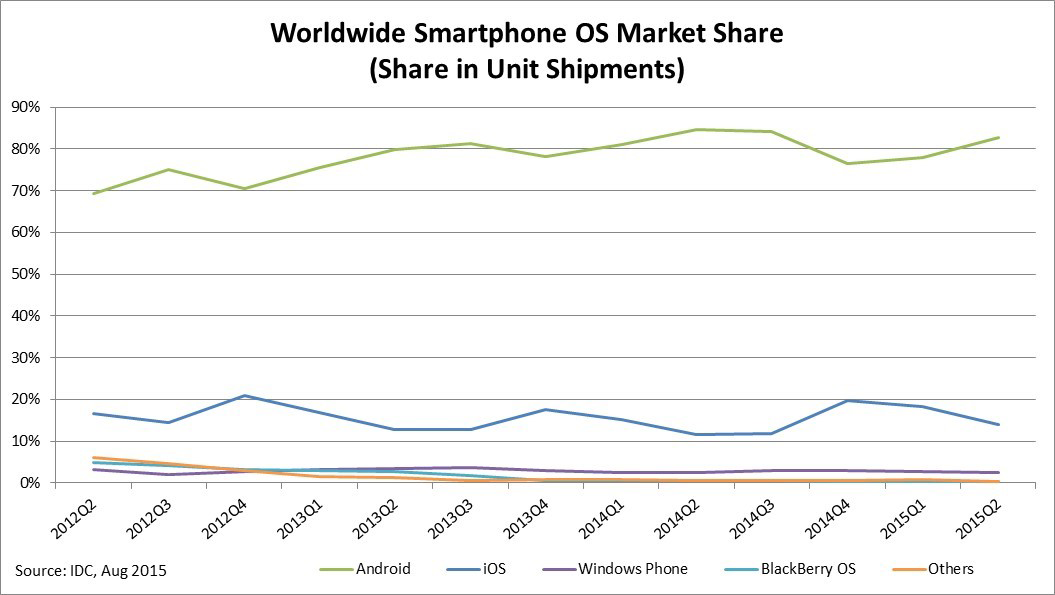
\includegraphics [scale=0.6]{imagens/smartphone-os-market-share.png}
    		\fonte{\citeonline{smartphone-os-market-share}}
  		\end{center}
	\end{figure}

\section{OBJETIVO} 
	
	Exemplo de seção.


\section{JUSTIFICATIVA}
	Exemplo de seção 3.

% ---
% Capitulo de revisão de literatura
% ---
\chapter{REVISÃO DA LITERATURA}
	
	Outro capítulo.

\section{SISTEMAS OPERACIONAIS MÓVEIS} % O título da seção deve ser em letras maiúsculas
	
	Exemplo de outra seção.
	
\subsection{iOS}
	
	Exemplo de subseção.


\subsubsection{Características}
	
	Exemplo de subsubseção.

% ---
% Procedimentos metodológicos
% ---
\chapter{PROCEDIMENTOS METODOLÓGICOS}
	
	Capítulo de Procedimentos Metodológicos.

\section{PROPOSTA} % O título da seção deve ser em letras maiúsculas
	
	Exemplo de seção.

\subsection{Requisitos Funcionais}
	
	Exemplo de subseção.

% ---
% Resultados
% ---
\chapter{RESULTADOS E DISCUSSÕES}

	Exemplo de capítulo de Resultados e Discussões.
	
\section{Aplicação}

	Exemplo de seção.

% ---
% Conclusão
% ---
\chapter{CONCLUSÃO}
	
	Exemplo de capítulo de conclusão.

% **************************************************

% ----------------------------------------------------------
% ELEMENTOS PÓS-TEXTUAIS
% ----------------------------------------------------------
% \postextual

% ----------------------------------------------------------
% Referências bibliográficas
% Arquivos que devem ser alterados
\bibliography{alterar/referencias}

% ----------------------------------------------------------
% Glossário
% ----------------------------------------------------------
%
% Consulte o manual da classe abntex2 para orientações sobre o glossário.
%
%\glossary

% ----------------------------------------------------------
% Apêndices
% ----------------------------------------------------------

% Informações que devem ser alteradas
% **************************************************
% ---
% Inicia os apêndices
% ---
\begin{apendicesenv}
\captionsetup[figure]{list=no}
\chapter{Cronograma}
	\setcounter{figure}{0} % Reinicia contagem das figuras do apêndice
	O trabalho foi desenvolvido com base nos cronogramas apresentados abaixo.
	\begin{figure}[H]
  		\begin{center}
    		\caption{Cronograma utilizado para o desenvolvimento do TCC1}
    		\label{cronograma1}
    		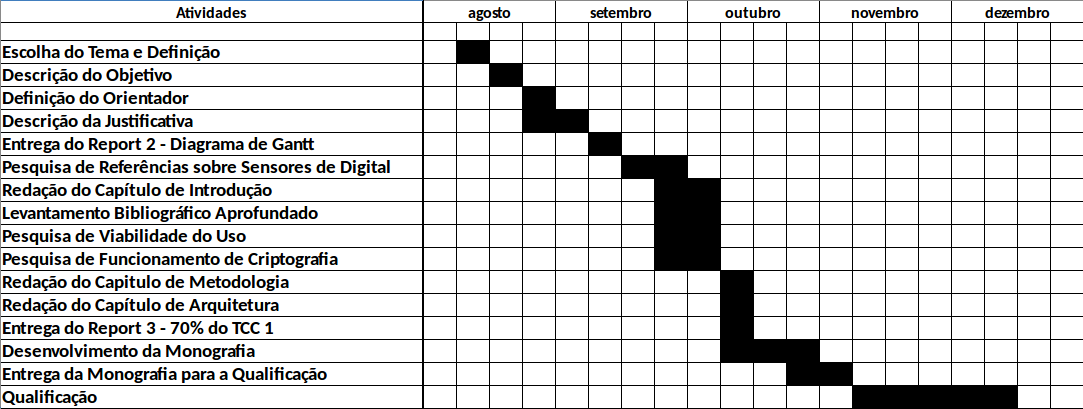
\includegraphics [scale=0.4]{imagens/cronograma1.png}
  		\end{center}
	\end{figure}

\chapter{Apêndice 2}
	Exemplos de listagem:
	
	\begin{itemize}  
		\item Item 1
		\item Item 2
		\item Item 3
	\end{itemize}


\chapter{Código fonte}

	Exemplo de código. O apêndice é opcional ao TCC e deve ser elaborado pelo próprio autor.

\scriptsize
\begin{lstlisting}
#include <stdio.h>

int main() {
  printf("Ola mundo !\n");
  return 0;
}
\end{lstlisting}

\end{apendicesenv}

% ----------------------------------------------------------
% Anexos
% ----------------------------------------------------------
\begin{anexosenv}

\chapter{Pesquisa IBGE}
O anexo é opcional ao TCC e são informações não elaboradas pelo próprio autor.

\end{anexosenv}

% Etiqueta para auxiliar contagem do numero de paginas do texto e dos elementos pos-textuais
\label{nropaginas}

% **************************************************

%---------------------------------------------------------------------
% INDICE REMISSIVO
%---------------------------------------------------------------------
\printindex

\end{document}
